Kimberling's Encyclopedia of Triangle Centers (ETC) \cite{etc} describes constructions and properties for thousands of such Centers, identified as $X_i$: $X_1$ for Incenter, $X_2$ for Barycenter, etc. Trilinear and/or Barycentric Coordinates are also provided for each Center. The former are signed distances to the sides of a triangle $T=P_1P_2P_3$, i.e. they are invariant with respect to similarity/reflection transformations, see Figure~\ref{fig:trilins}.

\begin{figure}
    \centering
    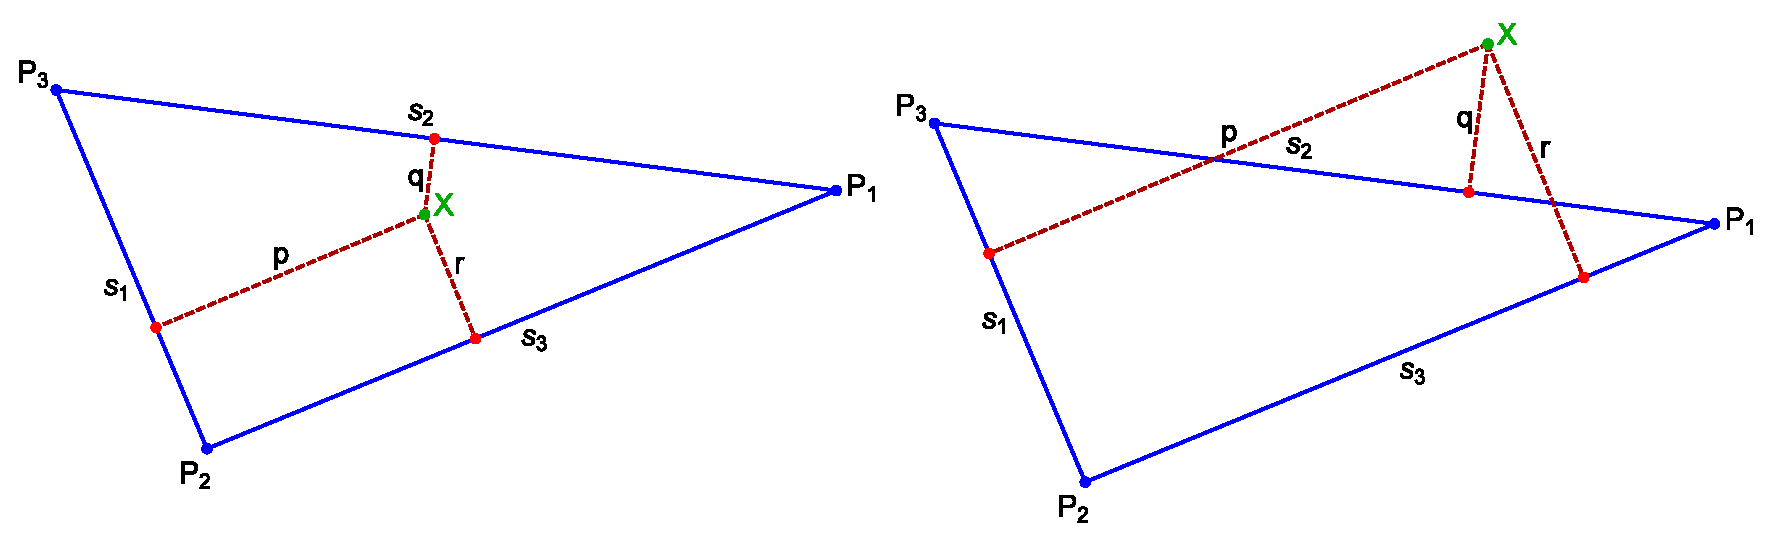
\includegraphics[width=\textwidth]{pics_1120_trilins.eps}
    \caption{Trilinear coordinates $p:q:r$ for a point $X$ on the plane of a generic triangle $T=P_1P_2P_3$ are homogeneous signed distances to each side whose lengths are $s_1,s_2,s_3$. The red dots are known as the {\em pedal points} of $X$ \cite{mw}. The left (resp. right) figure shows an interior (resp. exterior) point. In both cases $p,r$ are positive however $q$ is positive (resp. negative) in the former (resp. latter) case.}
    \label{fig:trilins}
\end{figure}

Trilinears can be easily converted to Cartesians using \cite{mw}:

\begin{equation}
\label{eqn:trilin-cartesian}
X=\frac{p s_1 P_1 + q s_2 P_2 + r s_3 P_3}{p{s_1}+q{s_2}+r{s_3}}
\end{equation}

\noindent where $s_1=|P_3-P_2|$, $s_2=|P_1-P_3|$ and $s_3=|P_2-P_1|$ are the sidelengths, Figure~\ref{fig:trilins}.
For instance, the Trilinears for the barycenter are $p = s_1^{-1},\,q = s_2^{-1},\,r = s_3^{-1}$, yielding the familiar $X_2 = (P_1+P_2+P_3)/3$.

%A point on the plane of a triangle $T=P_1P_2P_3$ can be defined by a triple $p:q:r$ of signed distances to each side\footnote{The Barycentrics of $p:q:r$ are $p\,s_1:q\,s_2:r\,s_3$ \cite{mw}.}, see Figure~\ref{fig:trilins}. This local coordinate system renders the point invariant under similarity transformations (rigid+dilation+reflection) of $T$.

A {\em Triangle Center} is such a triple obtained by applying a {\em Triangle Center Function} $h$ thrice to the sidelengths $s_1,s_2,s_3$ cyclically \cite{kimberling1993_rocky}:
 
\begin{equation}
\label{eqn:ftrilins}
    p:q:r {\iff} h(s_1,s_2,s_3):h(s_2,s_3,s_1):h(s_3,s_1,s_2)
\end{equation}

\noindent $h$ must (i) be {\em bi-symmetric}, i.e., $h(s_1,s_2,s_3)=h(s_1,s_3,s_2)$, and (ii) homogeneous, $h(t s_1, t s_2, t s_3)=t^n h(s_1,s_2,s_3)$ for some $n$ \cite{kimberling1993_rocky}.

Triangle Center Functions for a few Triangle Centers catalogued in \cite{mw} appears in Table~\ref{tab:center-trilinears}. Trilinears can be converted to Cartesians using \eqref{eqn:trilin-cartesian}.

\subsection{Constructions for Basic Triangle Centers}

Constructions for a few basic Triangle Centers are shown in Figure~\ref{fig:constructions}.

\begin{figure}
    \centering
    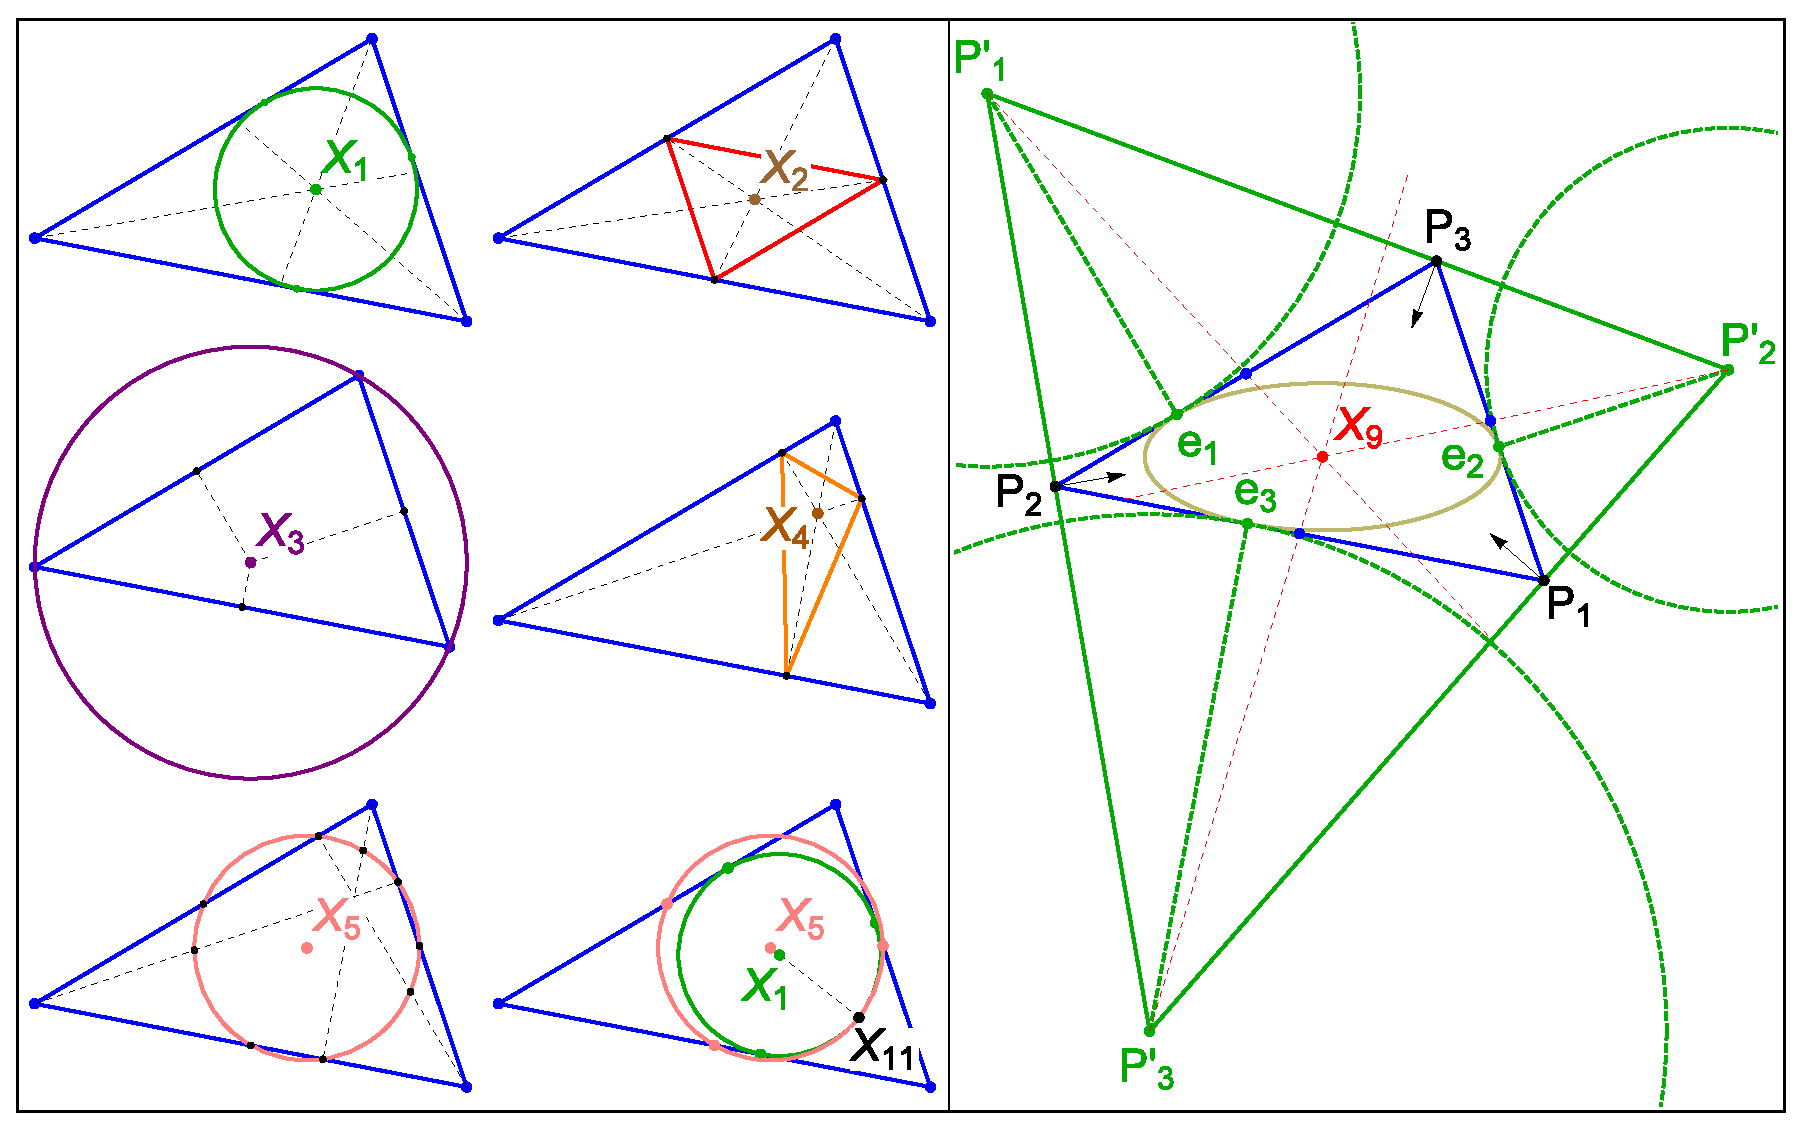
\includegraphics[width=\textwidth]{pics_1010_constr.eps}
    \caption{Constructions for Triangle Centers $X_i$, $i=1,2,3,4,5,9,11$, taken from \cite{reznik2020-intelligencer}.}
    \label{fig:constructions}
\end{figure}

\begin{itemize}
    \item The Incenter $X_1$ is the intersection of angular bisectors, and center of the Incircle (green), a circle tangent to the sides at three {\em Intouchpoints} (green dots), its radius is the {\em Inradius} $r$.
    \item The Barycenter $X_2$ is where lines drawn from the vertices to opposite sides' midpoints meet. Side midpoints define the {\em Medial Triangle} (red).
    \item The Circumcenter $X_3$ is the intersection of perpendicular bisectors, the center of the {\em Circumcircle} (purple) whose radius is the {\em Circumradius} $R$.
    \item The Orthocenter $X_4$ is where altitudes concur. Their feet define the {\em Orthic Triangle} (orange).
    \item $X_5$ is the center of the 9-Point (or Euler) Circle (pink): it passes through each side's midpoint, altitude feet, and Euler Points \cite{mw}.
    \item The Feuerbach Point $X_{11}$ is the single point of contact between the Incircle and the 9-Point Circle.
    \item Given a reference triangle $P_1P_2P_3$ (blue), the {\em Excenters} $P_1'P_2'P_3'$ are pairwise intersections of lines through the $P_i$ and perpendicular to the bisectors. This triad defines the {\em Excentral Triangle} (green).\
    \item The {\em Excircles} (dashed green) are centered on the Excenters and are touch each side at an {\em Extouch Point} $e_i,i=1,2,3$.
    \item Lines drawn from each Excenter through sides' midpoints (dashed red) concur at the {\em Mittenpunkt} $X_9$.
    \item Also shown (brown) is the triangle's {\em Mandart Inellipse}, internally tangent to each side at the $e_i$, and centered on $X_9$. This is identical to the $N=3$ Caustic.
\end{itemize}

\subsection{Derived Triangles}
\label{app:derived-tris}

A {\em Derived Triangle} $T'$ is constructed from the vertices of  a reference triangle $T$. A convenient representation is a 3x3 matrix, where each row, taken as Trilinears, is a vertex of $T'$. For example, the Excentral, Medial, and Intouch Triangles $T'_{exc}$, $T'_{med}$, and $T'_{int}$  are given by \cite{mw}: 

%, built from Triangle Center functions $h_1,h_2,h_3$ as follows \cite{kimberling1993_rocky}:

%\begin{align*}
%T'=
%\left[
%\begin{matrix}
%h_1(s_1,s_2,s_3) & h_2(s_1,s_2,s_3) & %h_3(s_1,s_2,s_3)\\ 
%   h_3(s_2,s_3,s_1) & h_1(s_2,s_3,s_1) & %h_2(s_2,s_3,s_1) \\
%   h_2(s_3,s_1,s_2) & h_3(s_3,s_1,s_2) & %h_1(s_3,s_1,s_2)
%\end{matrix}
%\right]
%\end{align*}

\begin{equation*}
\left[
\begin{matrix}
-1&1&1\\1&-1&1\\1&1&-1
\end{matrix}
\right],\;
\left[
\begin{matrix}
0&s_2^{-1}&s_3^{-1}\\s_1^{-1}&0&s_3^{-1}\\s_1^{-1}&s_2^{-1}&0
\end{matrix}
\right],\;
\left[
\begin{matrix}
0&\frac{s_1 s_3}{s_1-s_2+s_3}&\frac{s_1 s_2}{s_1+s_2-s_3}\\
\frac{s_2 s_3}{-s_1+s_2+s_3}&0&\frac{s_1 s_2}{s_1+s_2-s_3}\\
\frac{s_2 s_3}{-s_1+s_2+s_3}&\frac{s_1 s_3}{s_1-s_2+s_3}&0
\end{matrix}
\right]
\end{equation*}

A few Derived Triangles are shown in Figure~\ref{fig:derived-isosceles}, showing a property similar to Lemma~\ref{lem:axis-of-symmetry}, Appendix~\ref{app:method-lemmas}, namely, when the 3-periodic is an isosceles, one vertex of the Derived Triangle lies on the orbit's axis of symmetry.

\begin{figure}[H]
    \centering
    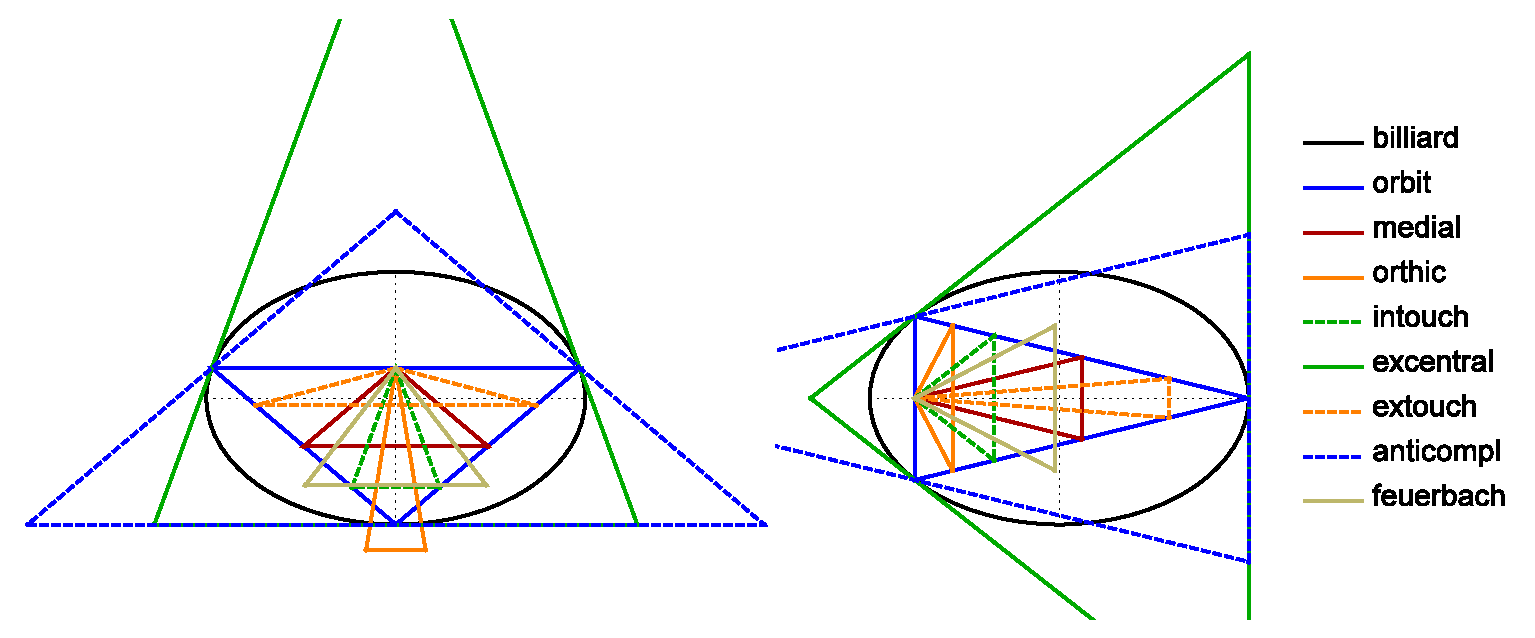
\includegraphics[width=\textwidth]{pics_1070_lemma3}
    \caption{When the orbit is an isosceles triangle (solid blue), any Derived Triangle will contain one vertex on the axis of symmetry of the orbit. \href{https://youtu.be/xyroRTEVNDc}{Video}}
    \label{fig:derived-isosceles}
\end{figure}



